\section{WebAssembly Specification}
\label{sec:wasm-specification}

The \gls{WebAssembly} standard is developed by W3C Working Group (WG) and W3C Community Group (CG) \cite{webassemblycommunitygroup_2023_webassembly}. The WebAssembly specification document \cite{webassemblycommunitygroup_2023_webassembly} focuses on Wasm's core Instruction Set Architecture layer, defining the instruction set, binary encoding, validation, execution semantics, and textual representation. However, it does not specify how WebAssembly programs interact with the execution environment or how they are invoked within that environment \cite{webassemblycommunitygroup_2023_webassembly}.


The WebAssembly specification gets extended through proposals. From creating a proposal to fully integrating it into WebAssembly core specification, it must process through several phases. Each proposal follows this progression \cite{webassemblyw3c_2023_webassembly}:
\begin{itemize}
  \item \textbf{0. Pre-Proposal [Individual]}: An individual files an issue on the design repository to discuss the idea. The idea is then discussed and championed by one or more members. 
  The proposal's general interest is voted on by the Community Group to ensure its scope and viability.
  \item \textbf{1. Feature Proposal [CG]}: A repository is created, and the champion works on reaching broad consensus within the Community Group. The design is iterated upon, and prototype implementations may be created to demonstrate the feature's viability.
  \item \textbf{2. Feature Description Available [CG + WG]}: A precise and complete overview document is produced with a high level of consensus. Prototype implementations create a comprehensive 
  test suite, but updates to the reference interpreter and spec document aren't yet required.
  \item \textbf{3. Implementation Phase [CG + WG]}: WebAssembly runtimes implement the feature, the spec document is updated with full English prose and formalization, and the reference interpreter is updated with a complete implementation. Toolchains implement the feature, and any remaining open questions are resolved.
  \item \textbf{4. Standardize the Feature [WG]}: The feature is handed over to the Working Group, which discusses the feature, considers edge cases, and confirms consensus on its completion. 
  The Working Group periodically polls on the feature's "ship-worthiness." If only minor changes are needed, they are made; otherwise, the feature is sent back to the Community Group.
  \item \textbf{5. The Feature is Standardized [WG]}: Once consensus is reached among Working Group members that the feature is complete, editors merge the feature into the main branch of the primary spec repository of WebAssembly.
\end{itemize}

Throughout these phases, proposals are refined, adjusted, and tested to ensure their seamless integration with the existing WebAssembly specification. The following \autoref{tab:active-proposals} lists the active proposals and their current phase. The proposal repository \cite{webassemblywg_2023_webassembly} contains more information about each proposal, including the proposal's current phase, champion, and links to the proposal's repository and design document, furthermore, the repository also contains a list of all the proposals that have been merged into the WebAssembly core specification.

In the next three sections, we will elaborate two proposals that have been already integrated into the WebAssembly core specification and one that is still an active proposal. The first proposal is the multi-value return, which allows functions to return multiple values a common feature in modern programming languages. The second proposal is the reference types, which allows WebAssembly to handle complex data types \cite{couriol_2020_webassembly}. The third proposal is the \gls{WebAssembly} GC proposal, which depends on the reference types proposal and adds garbage collection to WebAssembly and thereby expanding the range of languages that can be compiled to WebAssembly. These proposals were especially chosen because they make the WebAssembly target more accessible to a broader range of languages and use cases.

\begin{table}[htbp]
  \centering
  \begin{tabular}{|ll|}
    \hline
    \multicolumn{2}{|c|}{\textbf{Phase 5 - The Feature is Standardized (WG)}}                                                                                                                              \\ \hline
    \multicolumn{1}{|c|}{\textbf{Proposal}}                              &\multicolumn{1}{c|}{\textbf{Champion}}                                                                                          \\ \hline
    \multicolumn{2}{|l|}{\textit{\begin{tabular}[c]{@{}l@{}}Currently, there is no active Phase 5 proposal\\ that has not been merged into the Wasm Core spec.\end{tabular}}}                              \\ \hline
    \multicolumn{2}{|c|}{\textbf{Phase 4 - Standardize the Feature (WG)}}                                                                                                                                  \\ \hline
    \multicolumn{1}{|l|}{Tail call}                                      & Andreas Rossberg                                                                                                                \\ \hline
    \multicolumn{1}{|l|}{Extended Constant Expressions}                  & Sam Clegg                                                                                                                       \\ \hline
    \multicolumn{2}{|c|}{\textbf{Phase 3 - Implementation Phase (CG + WG)}}                                                                                                                                \\ \hline
    \multicolumn{1}{|l|}{Multiple memories}                              & Andreas Rossberg                                                                                                                \\ \hline
    \multicolumn{1}{|l|}{Custom Annotation Syntax in the Text Format}    & Andreas Rossberg                                                                                                                \\ \hline
    \multicolumn{1}{|l|}{Memory64}                                       & Sam Clegg                                                                                                                       \\ \hline
    \multicolumn{1}{|l|}{Exception handling}                             & Heejin Ahn                                                                                                                      \\ \hline
    \multicolumn{1}{|l|}{Web Content Security Policy}                    & Francis McCabe                                                                                                                  \\ \hline
    \multicolumn{1}{|l|}{Branch Hinting}                                 & Yuri Iozzelli                                                                                                                   \\ \hline
    \multicolumn{1}{|l|}{Relaxed SIMD}                                   & Marat Dukhan \& Zhi An Ng                                                                                                       \\ \hline
    \multicolumn{1}{|l|}{Typed Function References}                      & Andreas Rossberg                                                                                                                \\ \hline
    \multicolumn{1}{|l|}{Garbage collection}                             & Andreas Rossberg                                                                                                                \\ \hline
    \multicolumn{1}{|l|}{Threads}                                        & Conrad Watt                                                                                                                     \\ \hline
    \multicolumn{1}{|l|}{JS Promise Integration}                         & Ross Tate \& Francis McCabe                                                                                                    \\ \hline
    \multicolumn{1}{|l|}{Type Reflection for WebAssembly JavaScript API} & Ilya Rezvov                                                                                                                     \\ \hline
    \multicolumn{2}{|c|}{\textbf{Phase 2 - Proposed Spec Text Available (CG + WG)}}                                                                                                                        \\ \hline
    \multicolumn{1}{|l|}{ECMAScript module integration}                  & Asumu Takikawa \& Ms2ger                                                                                                        \\ \hline
    \multicolumn{1}{|l|}{Relaxed dead code validation}                   & Conrad Watt and Ross Tate                                                                                                       \\ \hline
    \multicolumn{1}{|l|}{Numeric Values in WAT Data Segments}            & Ezzat Chamudi                                                                                                                   \\ \hline
    \multicolumn{1}{|l|}{Instrument and Tracing Technology}              & Richard Winterton                                                                                                               \\ \hline
    \multicolumn{2}{|c|}{\textbf{Phase 1 - Feature Proposal (CG)}}                                                                                                                                         \\ \hline
    \multicolumn{1}{|l|}{Type Imports}                                   & Andreas Rossberg                                                                                                                \\ \hline
    \multicolumn{1}{|l|}{Component Model}                                & Luke Wagner                                                                                                                     \\ \hline
    \multicolumn{1}{|l|}{WebAssembly C and C++ API}                      & Andreas Rossberg                                                                                                                \\ \hline
    \multicolumn{1}{|l|}{Extended Name Section}                          & Ashley Nelson                                                                                                                   \\ \hline
    \multicolumn{1}{|l|}{Flexible Vectors}                               & Petr Penzin                                                                                                                     \\ \hline
    \multicolumn{1}{|l|}{Call Tags}                                      & Ross Tate                                                                                                                       \\ \hline
    \multicolumn{1}{|l|}{Stack Switching}                                & Francis McCabe \& Sam Lindley                                                                                                   \\ \hline
    \multicolumn{1}{|l|}{Constant Time}                                  & \begin{tabular}[c]{@{}l@{}}Sunjay Cauligi, Garrett Gu, \\ John Renner, Hovav Shacham, \\ Deian Stefan \& Conrad Watt\end{tabular} \\ \hline
    \multicolumn{1}{|l|}{JS Customization for GC Objects}                & Asumu Takikawa                                                                                                                  \\ \hline
    \multicolumn{1}{|l|}{Memory control}                                 & Deepti Gandluri                                                                                                                 \\ \hline
    \multicolumn{1}{|l|}{Reference-Typed Strings}                        & Andy Wingo                                                                                                                      \\ \hline
    \multicolumn{1}{|l|}{Profiles}                                       & Andreas Rossberg                                                                                                                \\ \hline
    \multicolumn{2}{|c|}{\textbf{Phase 0 - Pre-Proposal (CG)}}                                                                                                                                                      \\ \hline
    \multicolumn{2}{|l|}{\textit{Currently, there is no active pre-proposal.}}                                                                                                                    \\ \hline
  \end{tabular}
  \caption{Active proposals in the WebAssembly CG and WG obtained from \cite{webassemblywg_2023_webassembly}}
  \label{tab:active-proposals}
\end{table}


\section{Multi-Value Return}
\label{sec:multi-value-return}

In modern programming languages that support tuples, like Kotlin, Rust or Python, developers can effortlessly bundle several values into a single structure for returning from a function. 
Simple tasks, such as switching a pair of values or sorting an array, become challenging since they must be performed within the linear memory block. 
Some arithmetic functions, including modular operations and carry bits, can also yield multiple values.

Aside from functions that return tuples or multiple values, another limitation in the \hbox{WebAssembly} MVP was that loops and conditional blocks, in the code base cannot process or return more than one result \cite{sletten_2021_webassembly}. 
It would be equally intriguing to exchange values, perform arithmetic with overflow, or receive a multi-value tuple response in these scenarios as well. 
Furthermore, compilers are no longer required to jump through hoops when generating multiple stack values for core WebAssembly. This results in smaller generated bytecode and consequently, faster loading times and brings an extension type which is common in some programming languages like Rust or Python. Currently, the proposal has been already integrated into the WebAssembly core specification \cite{webassemblywg_2023_webassembly}. 

This proposal introduces a new type of arithmetic instruction "i32.divmod" \cite{fitzgerald_2019_multivalue, webassemblycommunitygroup_2023_webassembly} which takes a numerator and divisor and returns the quotient and remainder. Moreover, it enables multiple values to stay on the stack without needing to be copied into linear memory.

The most effective way to demonstrate the proposal is by presenting a straightforward example. In example \ref{code:multi-values}, we have a WAT file with an exported function called "reverseSub" that subtracts the second parameter from the first one and returns the result. 

Firstly, we define a module that contains two functions. The first one is an internal function called "swap" that takes two i32 (32-bit integer) parameters and returns them in reverse order. The second function is the one that we want to export and is called "reverseSub". It takes two 32 bit integer (i32) parameters and returns an integer (i32) result value. An exported function, means it will be accessible outside the WebAssembly module. Notice that "local.get 0" and "local.get 1" instructions are used to get the first and second parameters respectively. The "call \$swap" instruction calls the "swap" function and passes the two parameters to it. Finally, the "i32.sub" instruction \cite{webassemblycommunitygroup_2023_webassembly} subtracts the second parameter from the first one and returns the result.

\begin{lstlisting}[frame=lines, style=Wasm, caption={A Wasm module with a reverse subtraction function returning multiple values}, showstringspaces=false, captionpos=b, label=code:multi-values]
(module ;; reverseSub.wat
  (func $swap (param i32 i32) (result i32 i32)
    local.get 1
    local.get 0)

  (func (export "reverseSub") (param i32 i32) (result i32)
    local.get 0
    local.get 1
    call $swap
    i32.sub)
)
\end{lstlisting}

\section{Reference Types}
\label{sec:reference-types}

Before the introduction of reference types, WebAssembly only supported four primitive value types \cite{webassemblycommunitygroup_2023_webassembly}: 32-bit integers, 64-bit integers, 32-bit floating-points, and 64-bit floating-point numbers. With the introduction of reference types, WebAssembly capabilities are extended to include garbage-collected references. This will enable other proposals \cite{couriol_2020_webassembly} such as the garbage collection proposal, type import proposal (see \autoref{tab:active-proposals}) and more to utilize reference types without the need for glue code or dangerous workarounds. 

For instance, as Nick Fitzgerald noted in his publication \cite{fitzgerald_2020_webassembly}, the host stores objects in a side table and passes the indexes to the Wasm module. The Wasm module then uses these indexes to retrieve the objects from the side table. The usage of side tables requires glue code and is error-prone. Moreover, the glue code needs to be written in the host's language, making the Wasm module less portable.

The reference types proposal makes it possible for the host to specify and pass opaque handles to WebAssembly modules. These handles can be used to reference objects in the host environment, such as DOM nodes of a web page, a file handle or even open connection to a database. 

The reference types proposal brings three new features:
\begin{itemize}
    \item Makes it possible to have a \texttt{externref} type which is a opaque and unforgable reference to a object in the host environment.
    \item Makes it possible to store \texttt{externref} values in Wasm tables.
    \item Makes it possible to manipulate table entities with the help of new instructions.
\end{itemize}

As mentioned in the first bullet point, \texttt{externref} has two beneficial properties that fits the sandbox model of WebAssembly:
\begin{itemize}
    \item \textbf{Opaque}: The \texttt{externref} type is opaque, meaning that the reference does not reveal any significant information about the object it is referencing or the memory layout of the host environment.
    \item \textbf{Unforgable}: The \texttt{externref} type is unforgable, meaning it can either return a null reference or the same reference that was passed to the Wasm module. This prevents the Wasm module from creating new references to objects in the host environment. It makes it impossible to forge the reference. 
\end{itemize}

%TODO: Add example of how to use reference types

\section{Garbage Collection Proposal (Wasm GC)}
\label{sec:gc-proposals}

The garbage collection proposal \cite{webassemblycommunity_2023_gc} is currently under active development. This is one of the most anticipated proposals since it will enable developers to use managed-memory languages such as Kotlin, Java, Dart and many more to the WebAssembly ecosystem. 

Prior to this proposal, managed-memory languages have to ship and instantiate their own garbage collector every time the app loads, thus, increasing the \gls{WebAssembly} module size and increasing the startup time, even when every standard browser already has a garbage collector. \autoref{fig:wasm-gc-1} illustrates this problem, marked as "\#1 bloat problem", very well. Another issue is the fact that developers need to know how large the heap is going to be, to avoid running out of memory. A typical thing todo is to allocate a large amount of memory and hope that it is enough. This architecture treats the Wasm module as a separate entity from the host environment, even though it might reference objects in the host environment. This brings us to the next issue, marked as "\#2 split brain problem", there is no guarantee that the references in the JavaScript Heap are still valid, because there is no way to inform the garbage collector that the Wasm module is no longer using the reference or vice versa. This is a problem because the garbage collector might free the memory that the reference is pointing to, which will result in a dangling pointer. 

Even supposing that developers keep the references on the Wasm module side, there is still the possibility that we might need the JavaScript heap, due to the fact that the Wasm module might need to call Web APIs. Web APIs accept only JavaScript objects that live on the JavaScript heap. 
%
\begin{figure}[htbp]
  \centering
      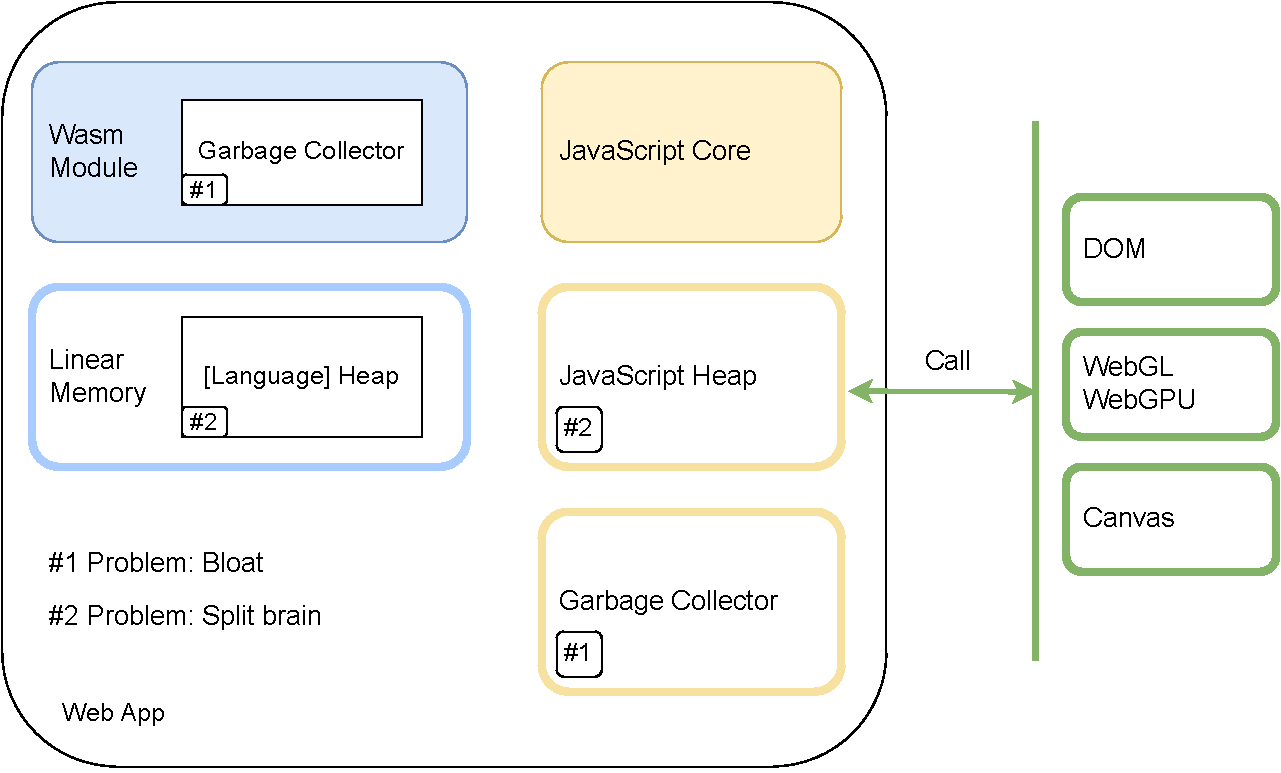
\includegraphics[width=1\linewidth]{images/wasm/wasm_gc_1.drawio.pdf}
  \caption{Wasm module without garbage collection proposal based on \cite{sekhar_2023_mobile}}
  \label{fig:wasm-gc-1}
\end{figure}
%
The Wasm GC proposal makes it possible to have a joint heap between JavaScript and WebAssembly GC code. This way the managed-memory code can allocate objects on the joint heap and when the JavaScript garbage collector runs, it will also collect the WebAssembly GC memory, because they are using the same heap memory (see \autoref{fig:wasm-gc-2}). Furthermore, depending on the runtime implementation, the runtime can return the unused memory back to the operating system to ensure the efficiency and responsiveness of the application \cite{sekhar_2023_mobile}. 

This means that the Wasm module doesn't have to include it's own garbage collector, which will reduce the Wasm module size and startup time. Moreover, the Wasm module can easily grow or shrink the memory based on consumption. 

To summarize, according to Vivek Sekhar in Wasm I/O 2023 conference, the garbage collection proposal brings the following three benefits \cite{sekhar_2023_mobile}:
%
\begin{itemize}
  \item \textbf{Smaller binaries for managed-memory languages}: Languages with dedicated garbage collectors no longer need to ship the garbage collector with the runtime. The hosts garbage collector can be used to garbage collect JavaScript and WebAssembly memory.
  \item \textbf{Enhanced interoperability with JavaScript code and Web APIs}: Wasm modules can directly access Web APIs, such as DOM, WebGL, Canvas, and more. Furthermore, objects can be passed to the JavaScript code, eliminating the need to copy objects between JavaScript and WebAssembly memories.
  \item \textbf{Resizable memory footprint}: The memory footprint can adjust to the usage and therefore additional memory can be allocated to WasmGC module. Unused memory can be returned to the host environment.
\end{itemize}
%
\begin{figure}[htbp]
  \centering
      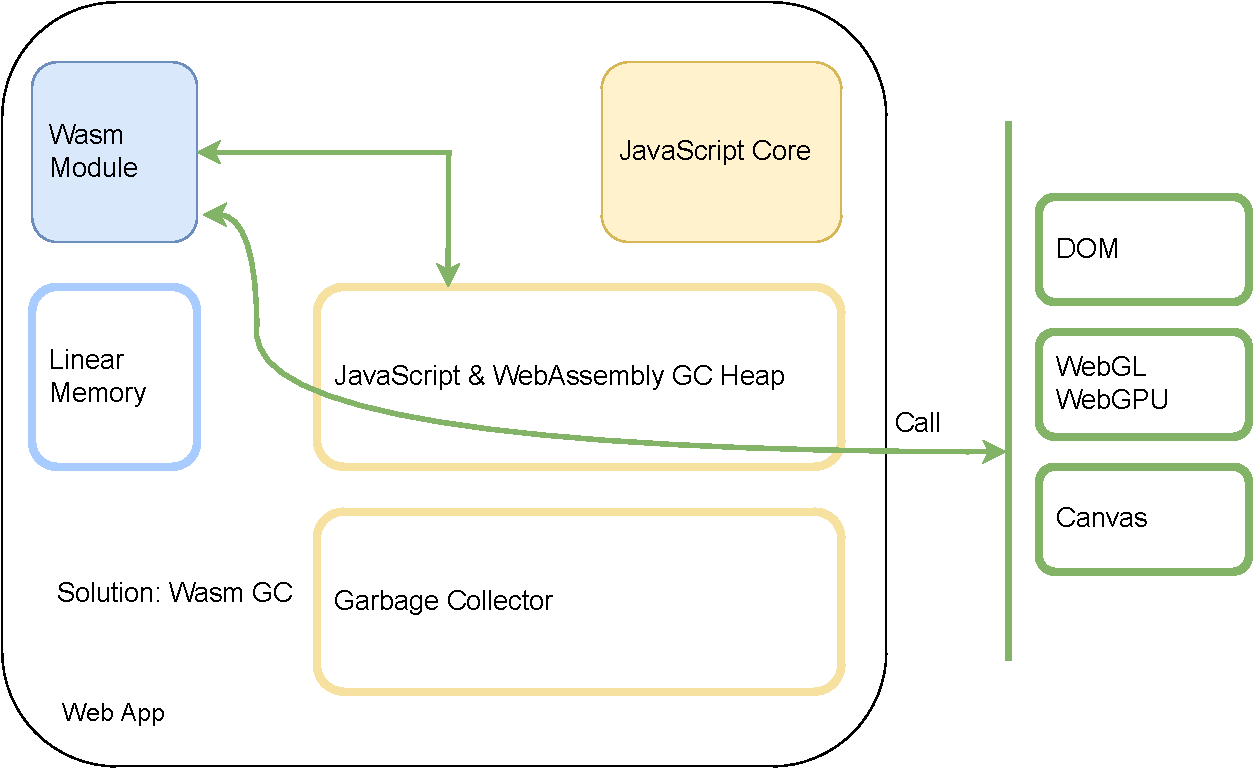
\includegraphics[width=1\linewidth]{images/wasm/wasm_gc_2.drawio.pdf}
  \caption{Wasm module with garbage collection proposal based on \cite{sekhar_2023_mobile}}
  \label{fig:wasm-gc-2}
\end{figure}
%
Even though the garbage collection proposal is still under active development, the Kotlin team has already rolled out an experimental compiler based on the proposal \cite{kotlin_2023_kotlin}.
